\localauthor{Thomas Kirz}

\subsection{Hochladen einer Revision}\label{subsec:sequenz-revision-hochladen}

Abbildung~\ref{fig:upload-revision-sequence} zeigt die Interaktionen zwischen den Klassen beim Ablehnen einer Einreichung.

\begin{figure}[H]
    \centering
    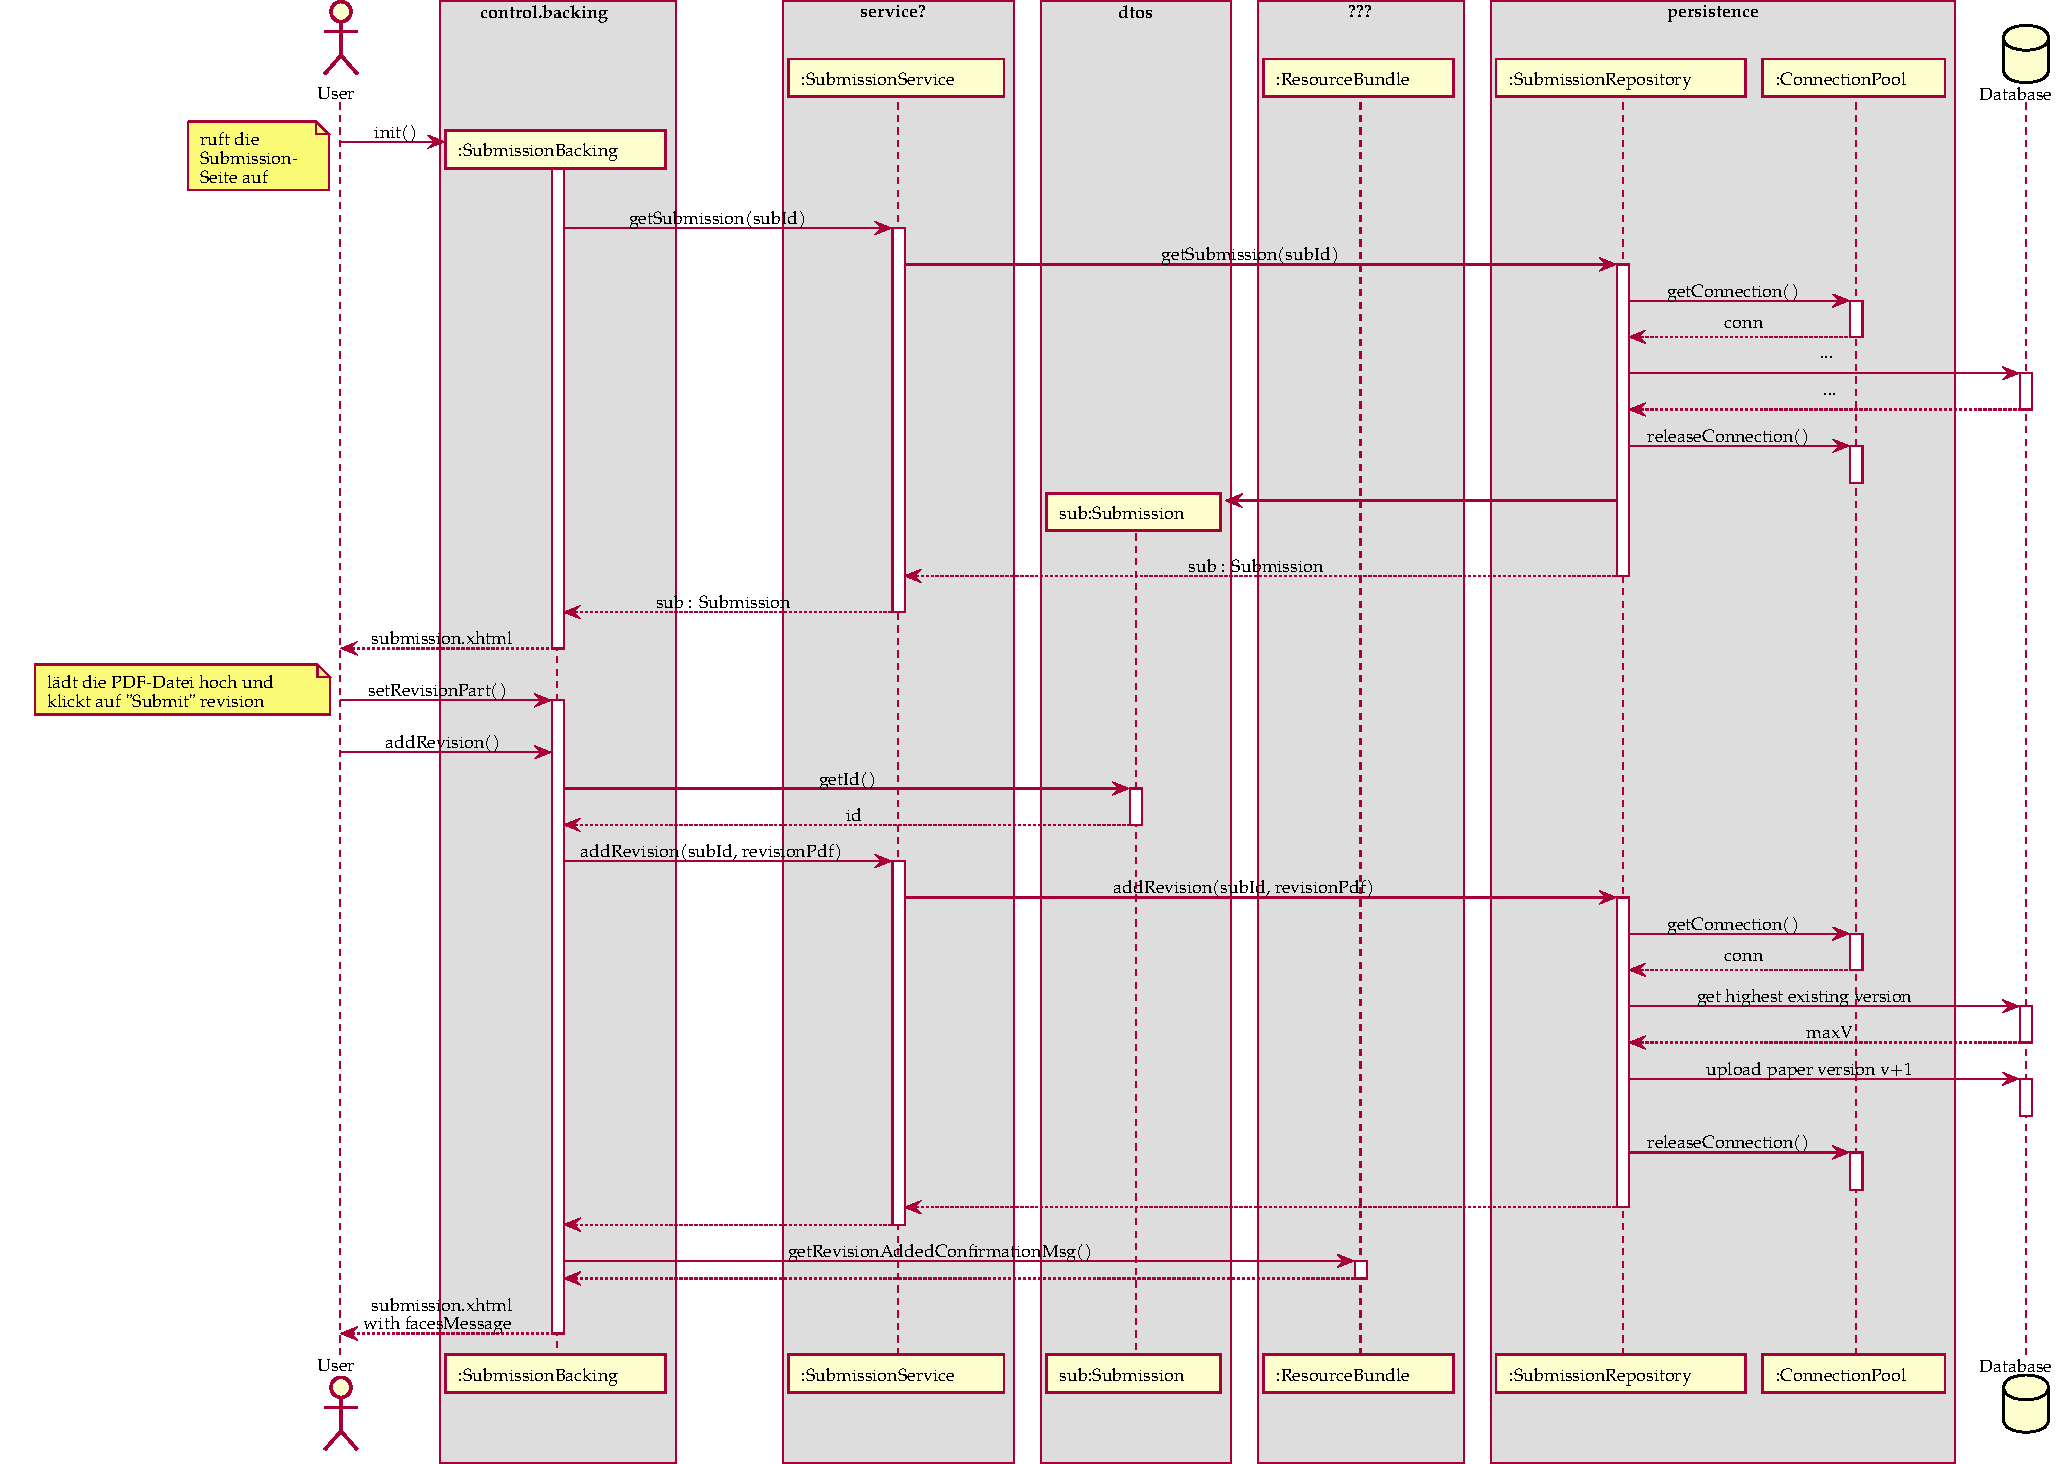
\includegraphics[width=0.8\textwidth]{graphics/upload_revision}
    \caption{Sequenzdiagramm zur Ablehnung einer Einreichung}
    \label{fig:upload-revision-sequence}
\end{figure}

\subsection{Ablehnung einer Einreichung}\label{subsec:sequenz-ablehnung}

Abbildung~\ref{fig:rejection-sequence} zeigt die Interaktionen zwischen den Klassen beim Ablehnen einer Einreichung, die Verbindung zum Datenbankserver schlägt aber fehl und die Einreichung kann nicht verändert werden. Es werden Exceptions bis zum Backing Bean geworfen und der Nutzer wird über den Fehler benachrichtigt.

\begin{figure}[H]
    \centering
    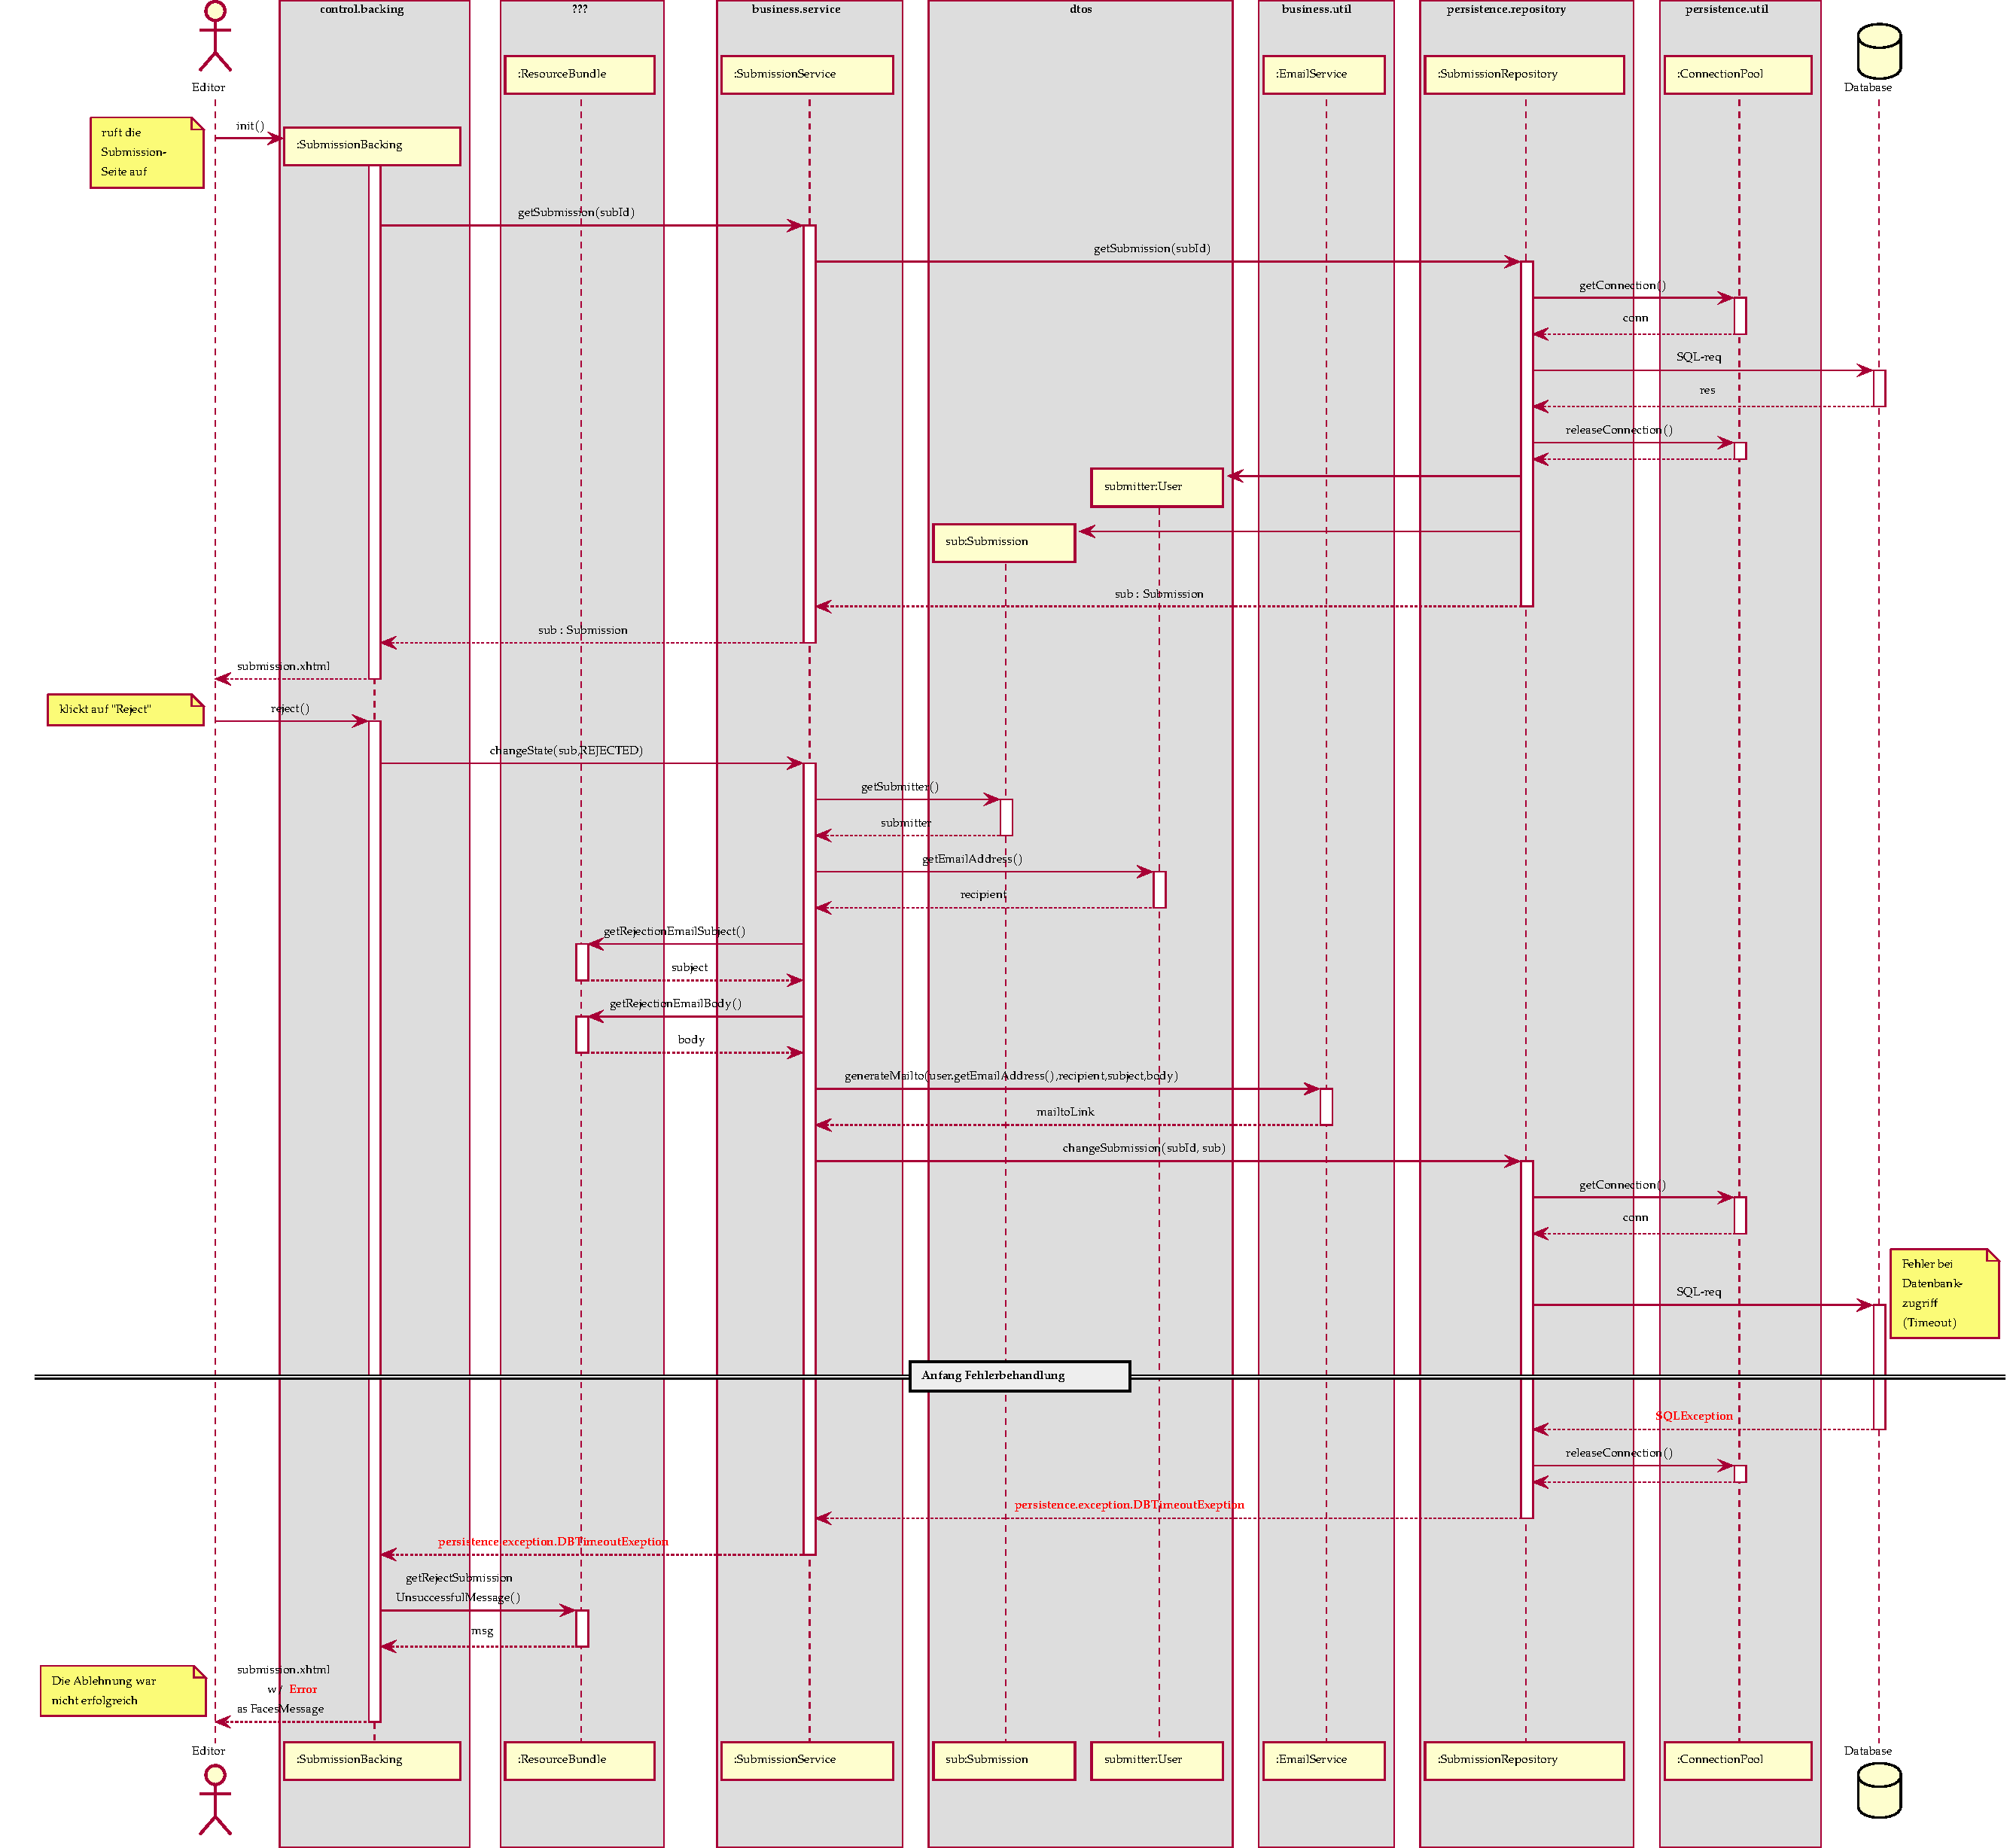
\includegraphics[width=0.8\textwidth]{graphics/reject_submission}
    \caption{Sequenzdiagramm zur Ablehnung einer Einreichung}
    \label{fig:rejection-sequence}
\end{figure}
